\section{Generation of Waypoints}
We first address the issue of finding a discrete set of waypoints, referenced above as $R$. We chose to formulate the problem using a discrete set of waypoints, rather than deal with the case of treating the region as continuous space, since it is much easier to accurately record sensor data at a given point. Discretising the space also allows the problem to be formulated in a manner that is easier to tackle, without losing the key aspects.
%\begin{itemize}
    %\item It is more straightforward to describe the problem using a discrete set of points rather than a continuous one.
%    \item It is much easier to process sensor information if it is known exactly where this data has been captured. The UAVs may stop at each discrete waypoint to visit these locations. *Focus on this point, expand if possible*
%    \item The case of path-finding using discrete waypoints has a strong body of literature behind it
%    \item The UAVs run autopilot software which can guide them using the on-board GPS sensor
%\end{itemize}

%which are the center points of cells that partition the region of interest.
\note{set of waypoints create a voronoi partition, might be worth talking about}

\note{Above needs revision, will come back once rest of chapter has been fleshed out a bit more}
We began by assuming that the region which is to be surveyed, the \textit{region of interest}, can be described by a polygon on the x-y plane, since it allows for a discrete representation. We favour a discrete representation since it is computationally much easier to record and manipulate a set of points denoting the boundary rather than an arbitrary curve. Given this polygon, the goal is to generate a set of points, $R$, which are a uniform distance from each other in the x and y directions and lie inside the polygonal grid. These points form a regular tessellation of the region of interest. In order to do this, we employed the following methodology, using well-known algorithms:
\begin{enumerate}
    \item Find the rectangle that tightly bounds the polygon, which is oriented with the x-y plane. This is shown in \ref{fig:PolygonWithBoundingRect}
    \item Generate a set of grid points in the bounding rectangle. This is shown in \ref{fig:PolygonWithBoundingRectAndGridPoints}
    \item Prune the points that lie inside the rectangle but outside the polygon. This is shown in \ref{fig:PolygonWithBoundingRectAndGridPointsPruned}
\end{enumerate}


\begin{figure}
\centering
\subfloat[Arbitrary Polygonal Region]{
  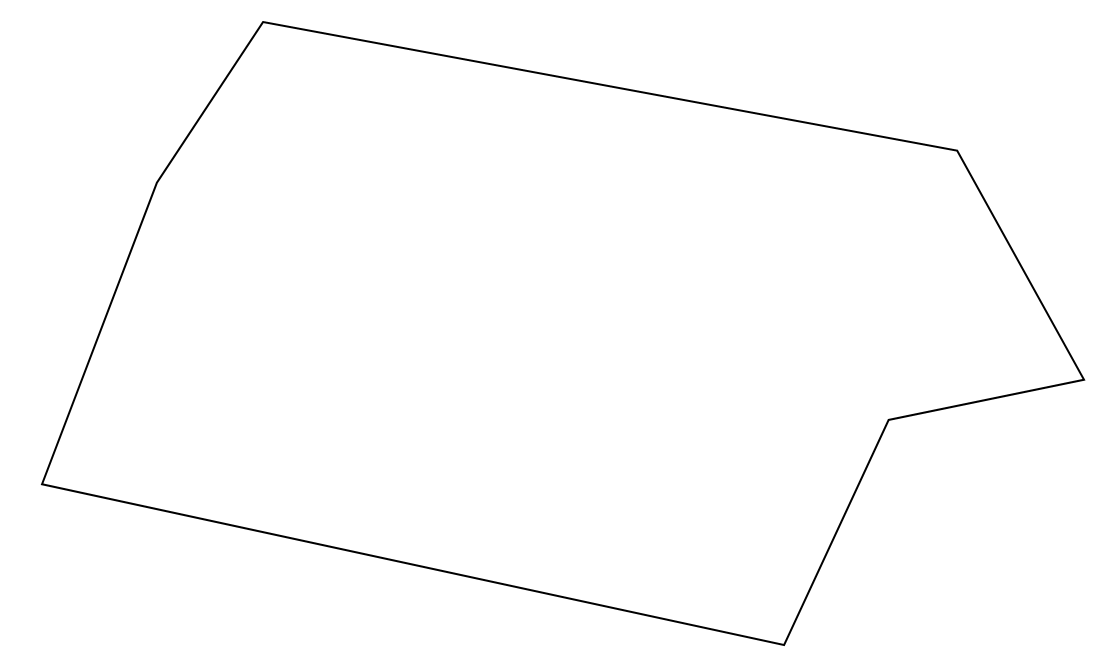
\includegraphics[width=65mm]{Chapters/MultiAgentCoverage/Figs/Polygon.PNG}\label{fig:PolygonOnly}
}
\subfloat[Bounding Rectangle Found]{
  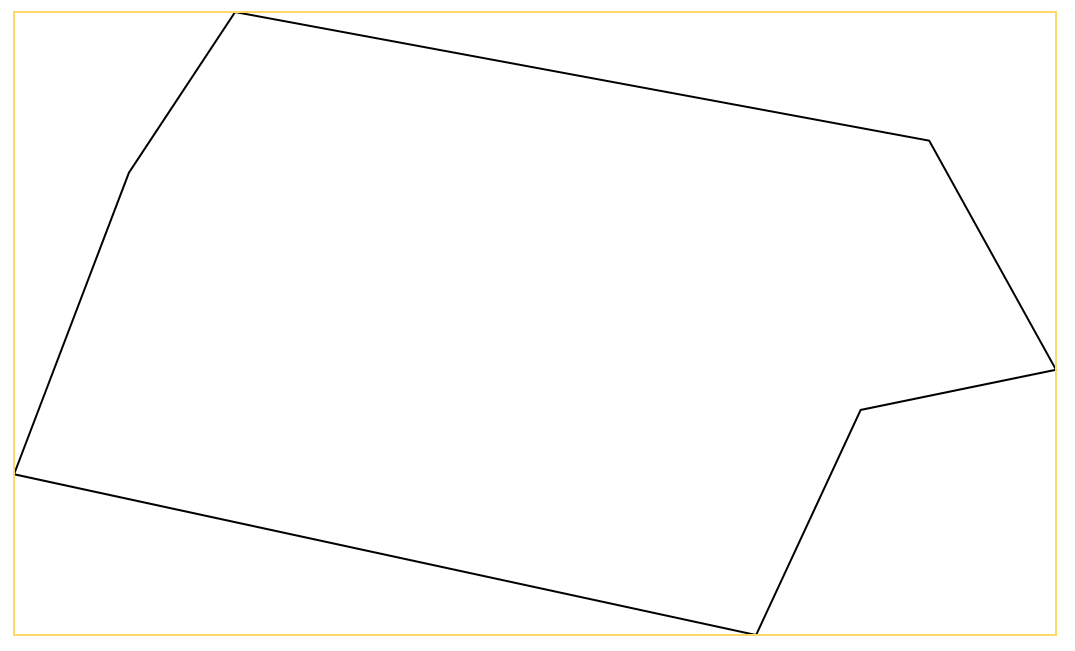
\includegraphics[width=65mm]{Chapters/MultiAgentCoverage/Figs/PolygonBoundingRect.PNG}\label{fig:PolygonWithBoundingRect}
}
\hspace{0mm}
\subfloat[Grid Points Generated in Bounding Rectangle]{
  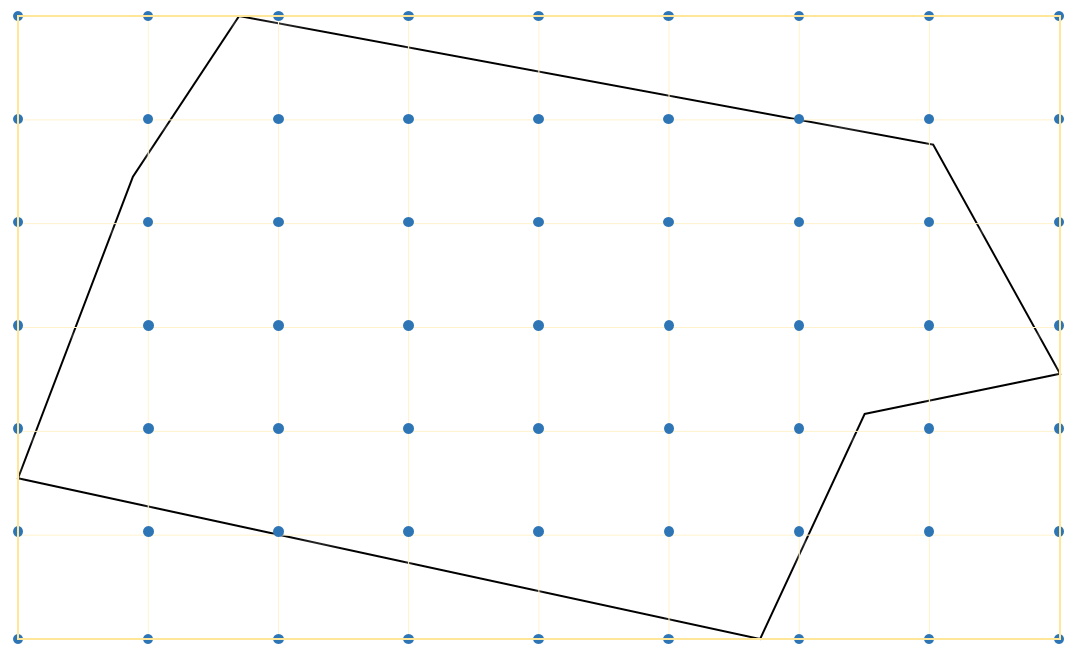
\includegraphics[width=65mm]{Chapters/MultiAgentCoverage/Figs/PolygonBoundingRectGridPoints.PNG}\label{fig:PolygonWithBoundingRectAndGridPoints}
}
\subfloat[Grid Points Outside of Polygon Pruned]{
  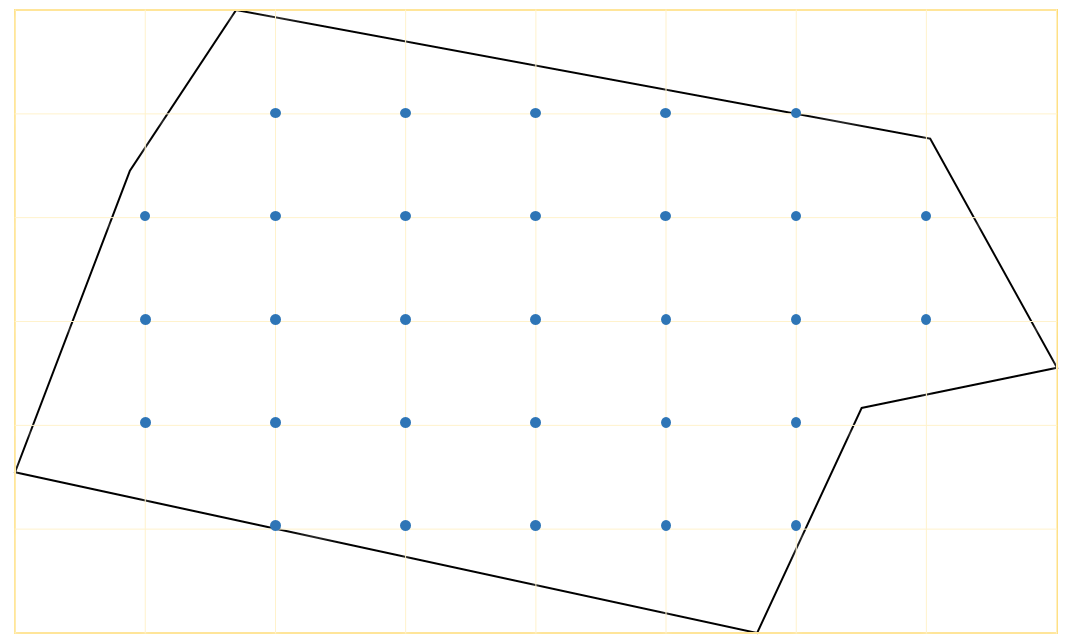
\includegraphics[width=65mm]{Chapters/MultiAgentCoverage/Figs/PolygonBoundingRectGridPointsPruned.PNG}\label{fig:PolygonWithBoundingRectAndGridPointsPruned}
}
\end{figure}

This procedure was devised with the aim of being straightforward to implement and modify. The algorithm used to carry out these steps is outlined in \ref{alg:GridGeneration}. 


Algorithm \ref{alg:PointInPolygon} outlines a procedure for finding whether a point is contained in a polygon using the well-known \textit{crossing test}, described in  \cite{Shimrat1962Algorithms}.



\begin{algorithm}{}
%\caption{Crossing Test for Point in Polygon based on \cite{Shimrat1962Algorithms}}
\caption{Point in Polygon}
\label{alg:PointInPolygon}
\begin{algorithmic}[1]
\renewcommand{\algorithmicrequire}{\textbf{Input:}}
\renewcommand{\algorithmicensure}{\textbf{Output:}}
%Input
\REQUIRE $ \newline R \quad \text{ The polygon which covers the region of interest}
%\newline R \quad \text{ The set of (x, y) points defining the polygon which covers the region of interest}
\newline P \quad \text{ A point which will be tested for containment in the polygon }
$
%Output
\ENSURE $\newline \text{True if P is contained in R else False }$

\hfill\pagebreak
\STATE polygon\_points $\leftarrow$ The set of points which define the edges of R
\IF{x coordinate of $P$ is greater than the largest value or less than the smallest value of the x coordinates of the points in $R$}
\RETURN False
\ELSIF{y coordinate of $P$ is greater than the largest value or less than the smallest value of the y coordinates of the points in $R$}
\RETURN False


%\ELSIF{x coordinate of P is less than the smallest value of the x coordinate of all the points in R}
%\RETURN false
%\ELSIF{y coordinate of P is greater than the largest value of the y coordinate of all the points in R}
%\RETURN false
%\ELSIF{y coordinate of P is less than the smallest value of the y coordinate of all the points in R}
%\RETURN false

\ELSE
\STATE point\_in\_polygon $\leftarrow$ True
\STATE edges $\leftarrow$ the set of edges defining
\FOR{each edge in edges}
\STATE p1 $\leftarrow$ the first point of edge
\STATE p2 $\leftarrow$ the second point of edge

\IF{(y coordinate of $P$ lies between y coordinates of p1 and p2) AND
     x coordinate of $P$ is less than the x coordinate of the point of intersection between e and the ray extended to +$\infty$ from $P$ in the +x direction}
\STATE point\_in\_polygon $\leftarrow$ not point\_in\_polygon
\ENDIF

\ENDFOR
\ENDIF
\end{algorithmic} 
\end{algorithm}


\begin{algorithm}{H}
\caption{Generate Grid Points In Polygon}
\label{alg:GridGeneration}
\begin{algorithmic}[1]
\renewcommand{\algorithmicrequire}{\textbf{Input:}}
\renewcommand{\algorithmicensure}{\textbf{Output:}}
%Input
\REQUIRE $ \newline R \quad\text{ The set of (x, y) points defining the polygon which covers the region of interest}
\newline x\_spacing \quad\text{ The desired spacing between points in the x direction}
\newline y\_spacing \quad\text{ The desired spacing between points in the y direction}
$
%Output
\ENSURE $\newline grid\_points \quad \text{ A set of uniformly spaced (x, y) points, which define a regular } \newline \text{ tessellation of the region of interest}$

\hfill\pagebreak
\STATE grid\_points $\leftarrow$ empty array

\STATE max\_x $\leftarrow$ maximum x value of all points in R
\STATE min\_x $\leftarrow$ minimum x value of all points in R
\STATE max\_y $\leftarrow$ maximum y value of all points in R
\STATE min\_y $\leftarrow$ minimum y value of all points in R

\STATE bounding\_rect $\leftarrow$ The tightest bounding rectangle which contains the polygon R defined by the points (min\_x, min\_y), (min\_x, max\_y), (max\_x, max\_y),(max\_x, min\_y).

\STATE no\_y\_points $\leftarrow \left \lceil{\frac{max_y - min_y}{y\_spacing}}\right \rceil$
\STATE no\_x\_points $\leftarrow \left \lceil{\frac{max_y - min_y}{x\_spacing}}\right \rceil$

\FOR{y\_spacing\_index = 0 to no\_y\_points}
\FOR{x\_spacing\_index = 0 to no\_x\_points}
\STATE Add (min\_x + x\_spacing * x\_spacing\_index, min\_y + y\_spacing * y\_spacing\_index) to grid\_points
\ENDFOR
\ENDFOR
\FOR{point in grid\_points}
\IF{Point in Polygon(R, point) is false}
\STATE Remove point from grid\_points
\ENDIF
\ENDFOR
\RETURN grid\_points
\end{algorithmic} 
\end{algorithm}


%From a practical perspective, the region specified is defined over the earth's surface, which is not planar. For small regions, it can be assumed that this region is planar, since at 

%The generation of grid points takes this into account. The earth can be well described mathematically as an ellipsoid talk about WGS84






